\documentclass[12pt]{article}[margin=1in]
\usepackage{fullpage,graphicx,psfrag,amsmath,amsfonts,verbatim}
\usepackage{multicol,multirow}
\usepackage[small,bf]{caption}
\usepackage{amsthm}
\usepackage{hyperref}
\usepackage{bbm} % for the indicator function to look good
\usepackage{color}
\usepackage{mathtools}
\usepackage{fancyhdr} % for the header
\usepackage{booktabs} % for regression table display (toprule, midrule, bottomrule)
\usepackage{adjustbox} % for regression table display
\usepackage{threeparttable} % to use table notes
\usepackage{natbib} % for bibliography
\input newcommand.tex
\bibliographystyle{apalike}
\setlength{\parindent}{0pt} % remove the automatic indentation % for problem set
\renewcommand{\thesection}{Question \arabic{section}}
\renewcommand{\thesubsection}{\arabic{section}.\arabic{subsection}}

% Settings for page number in the footer
\pagestyle{fancy}
\fancyhf{}
\fancyfoot[C]{\thepage}
\renewcommand{\headrulewidth}{0pt}
\renewcommand{\footrulewidth}{0pt}

\title{\textbf{Linear Regression Equation from DDC} \\
\vspace{.3cm}
\large Coding Exercise \\
Environmental Economics}
\author{Zixuan}
\date{\today}

\begin{document}
\maketitle

\section{Spatial Data}
\subsection{Irrigation in Almeria}
The \texttt{land\_use\_panel.csv} provides information on the use of land (crop type and irrigation) for each piece of land in Almeria. 

\begin{figure}[h]
    \centering
    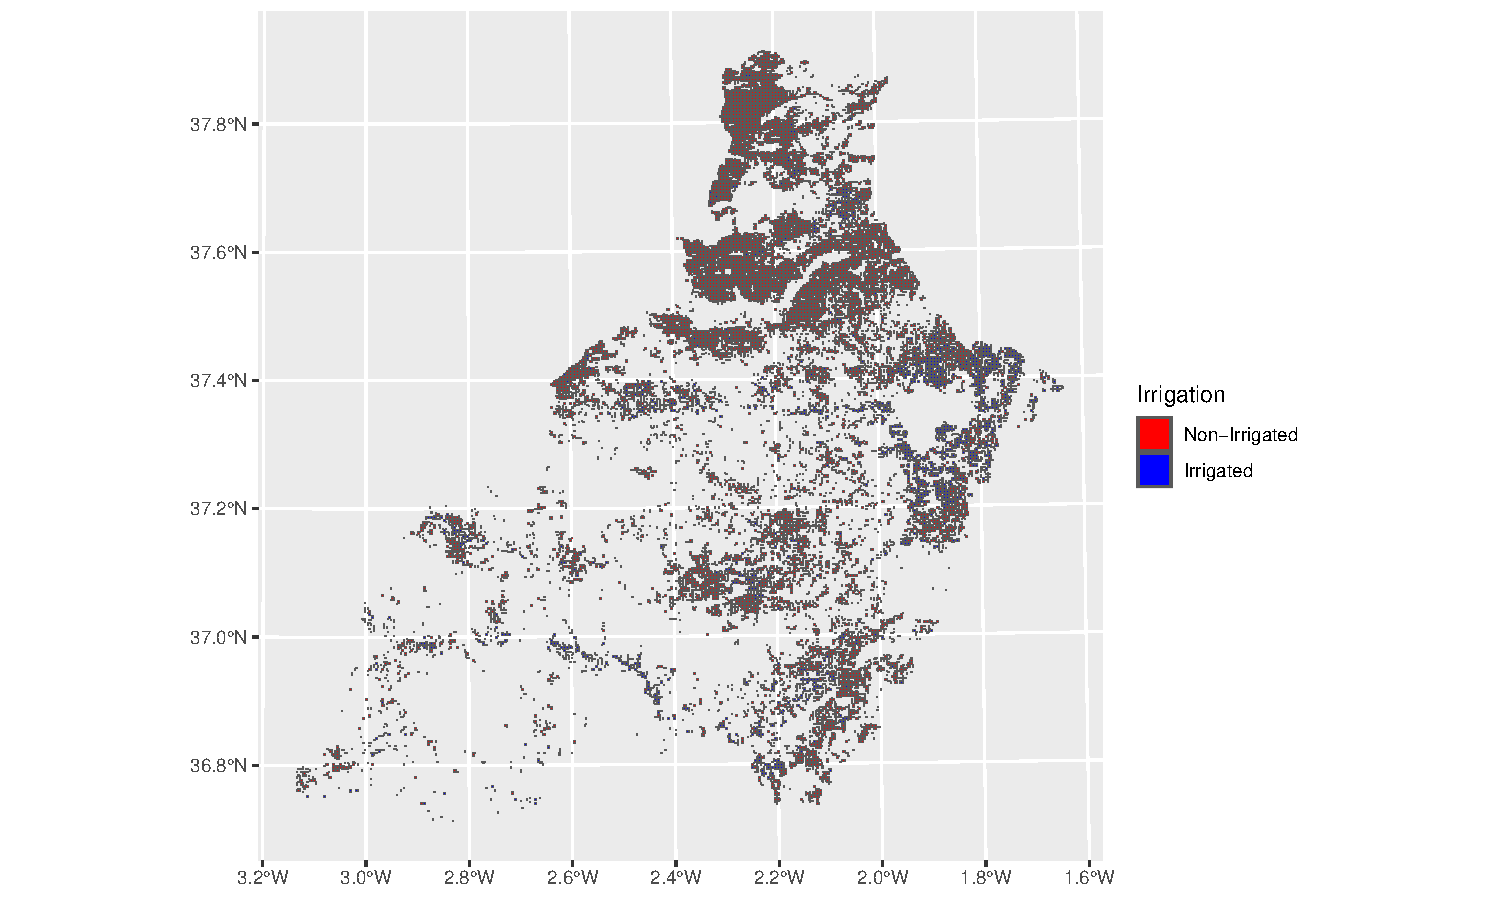
\includegraphics[width=0.8\textwidth]{../Figures/land_use_distribution_almeria_2021.pdf}
\end{figure}


\end{document}


